\documentclass{slide}
% \usepackage{pgfpages}

% \setbeameroption{show notes on second screen}

\title{Service-Based Architecture}
\subtitle{CSSE6400}
\author{Richard Thomas}
\date{\week{4}}

\begin{document}

\maketitle

\definition{Distributed System}{A system with multiple components located on different machines that communicate and coordinate actions in order to appear as a single coherent system to the end-user.}

\point[Quote]{A distributed system is one in which the failure of a computer you didn't even know existed can render your own computer unusable.\\
-- Leslie Lamport}
\note{Emphasise quality attributes and how architectural styles deliver those attributes.}

\begin{frame}{Microkernel Architecture}
Failure is the defining difference between distributed and local programming, so you have to design distributed systems with the expectation of failure. Imagine asking people, "If the probability of something happening is one in 1013, how often would it happen?" Common sense would be to answer, "Never." That is an infinitely large number in human terms. But if you ask a physicist, she would say, "All the time. In a cubic foot of air, those things happen all the time."

When you design distributed systems, you have to say, "Failure happens all the time." So when you design, you design for failure. It is your number one concern. What does designing for failure mean? One classic problem is partial failure. If I send a message to you and then a network failure occurs, there are two possible outcomes. One is that the message got to you, and then the network broke, and I just didn't get the response. The other is the message never got to you because the network broke before it arrived.

So if I never receive a response, how do I know which of those two results happened? I cannot determine that without eventually finding you. The network has to be repaired or you have to come up, because maybe what happened was not a network failure but you died. How does this change how I design things? For one thing, it puts a multiplier on the value of simplicity. The more things I can do with you, the more things I have to think about recovering from.
 -- https://www.artima.com/articles/designing-distributed-systems
\end{frame}
\note[itemize]{
    \item Monolith -- Commonly use method invocation to communicate with plug-ins
    \item Other message passing protocols may be used
}

\definition{Registry}{Tracks which plug-ins are available to the core system and how to access them.}
\note[itemize]{
    \item Monolith -- Registry can be simply plug-in name and reference to delegate object
    \item More detail about communication protocol and data structure required for other message passing approaches
}

\begin{frame}{Loading Plug-ins}
    \vspace{1mm}
    {\huge
    \begin{description}
        \item[Static Loading] when application starts
        \vspace{3mm}
        \item[Dynamic Loading] as needed at run-time
        \vspace{3mm}
        \item[Registry] designed for the selected strategy
    \end{description}
    }
\end{frame}
\note[itemize]{
    \item Dynamic loading requires a plug-in registration and de-registration interface
    \item Could mention that one of the reasons for JARs in Java was to allow dynamic loading of classes
}

\questionanswer{Can you think of a \highlight{microkernel archiecture}?}{Web Browser?}
\note[itemize]{
    \item Eclipse
    \item Operating Systems
    \begin{itemize}
        \item Some Unix variants
        \item Zircon - Google OS kernel
        \item Nintendo Switch OS
    \end{itemize}
    \item Insurance Claims Processing
    \item Payroll
    \item WordPress
}

\definition{Independent Plug-in Principle}{Plug-ins should be independent, with no dependencies on other plug-ins.
The only dependency on the core system is through the plug-in interface.}

\definition{Standard Interface Principle}{There should be a single interface that defines how the core system uses plug-ins.}

\questionanswer{Does a plug-in architecture equate to a microkernel archiecture?}{What about \highlight{IntelliJ}?}
\note{Not really a microkernel, just a large IDE that allows plug-ins.}

\begin{frame}{Plug-ins with Separate Databases}
    \begin{itemize}
        \LARGE\item Plug-ins cannot access core system data
        \begin{itemize}
            \Large\item Core system may pass data to the plug-in
        \end{itemize}
        \LARGE\item Plug-ins may have their own persistent data
    \end{itemize}
    \vspace{1cm}
    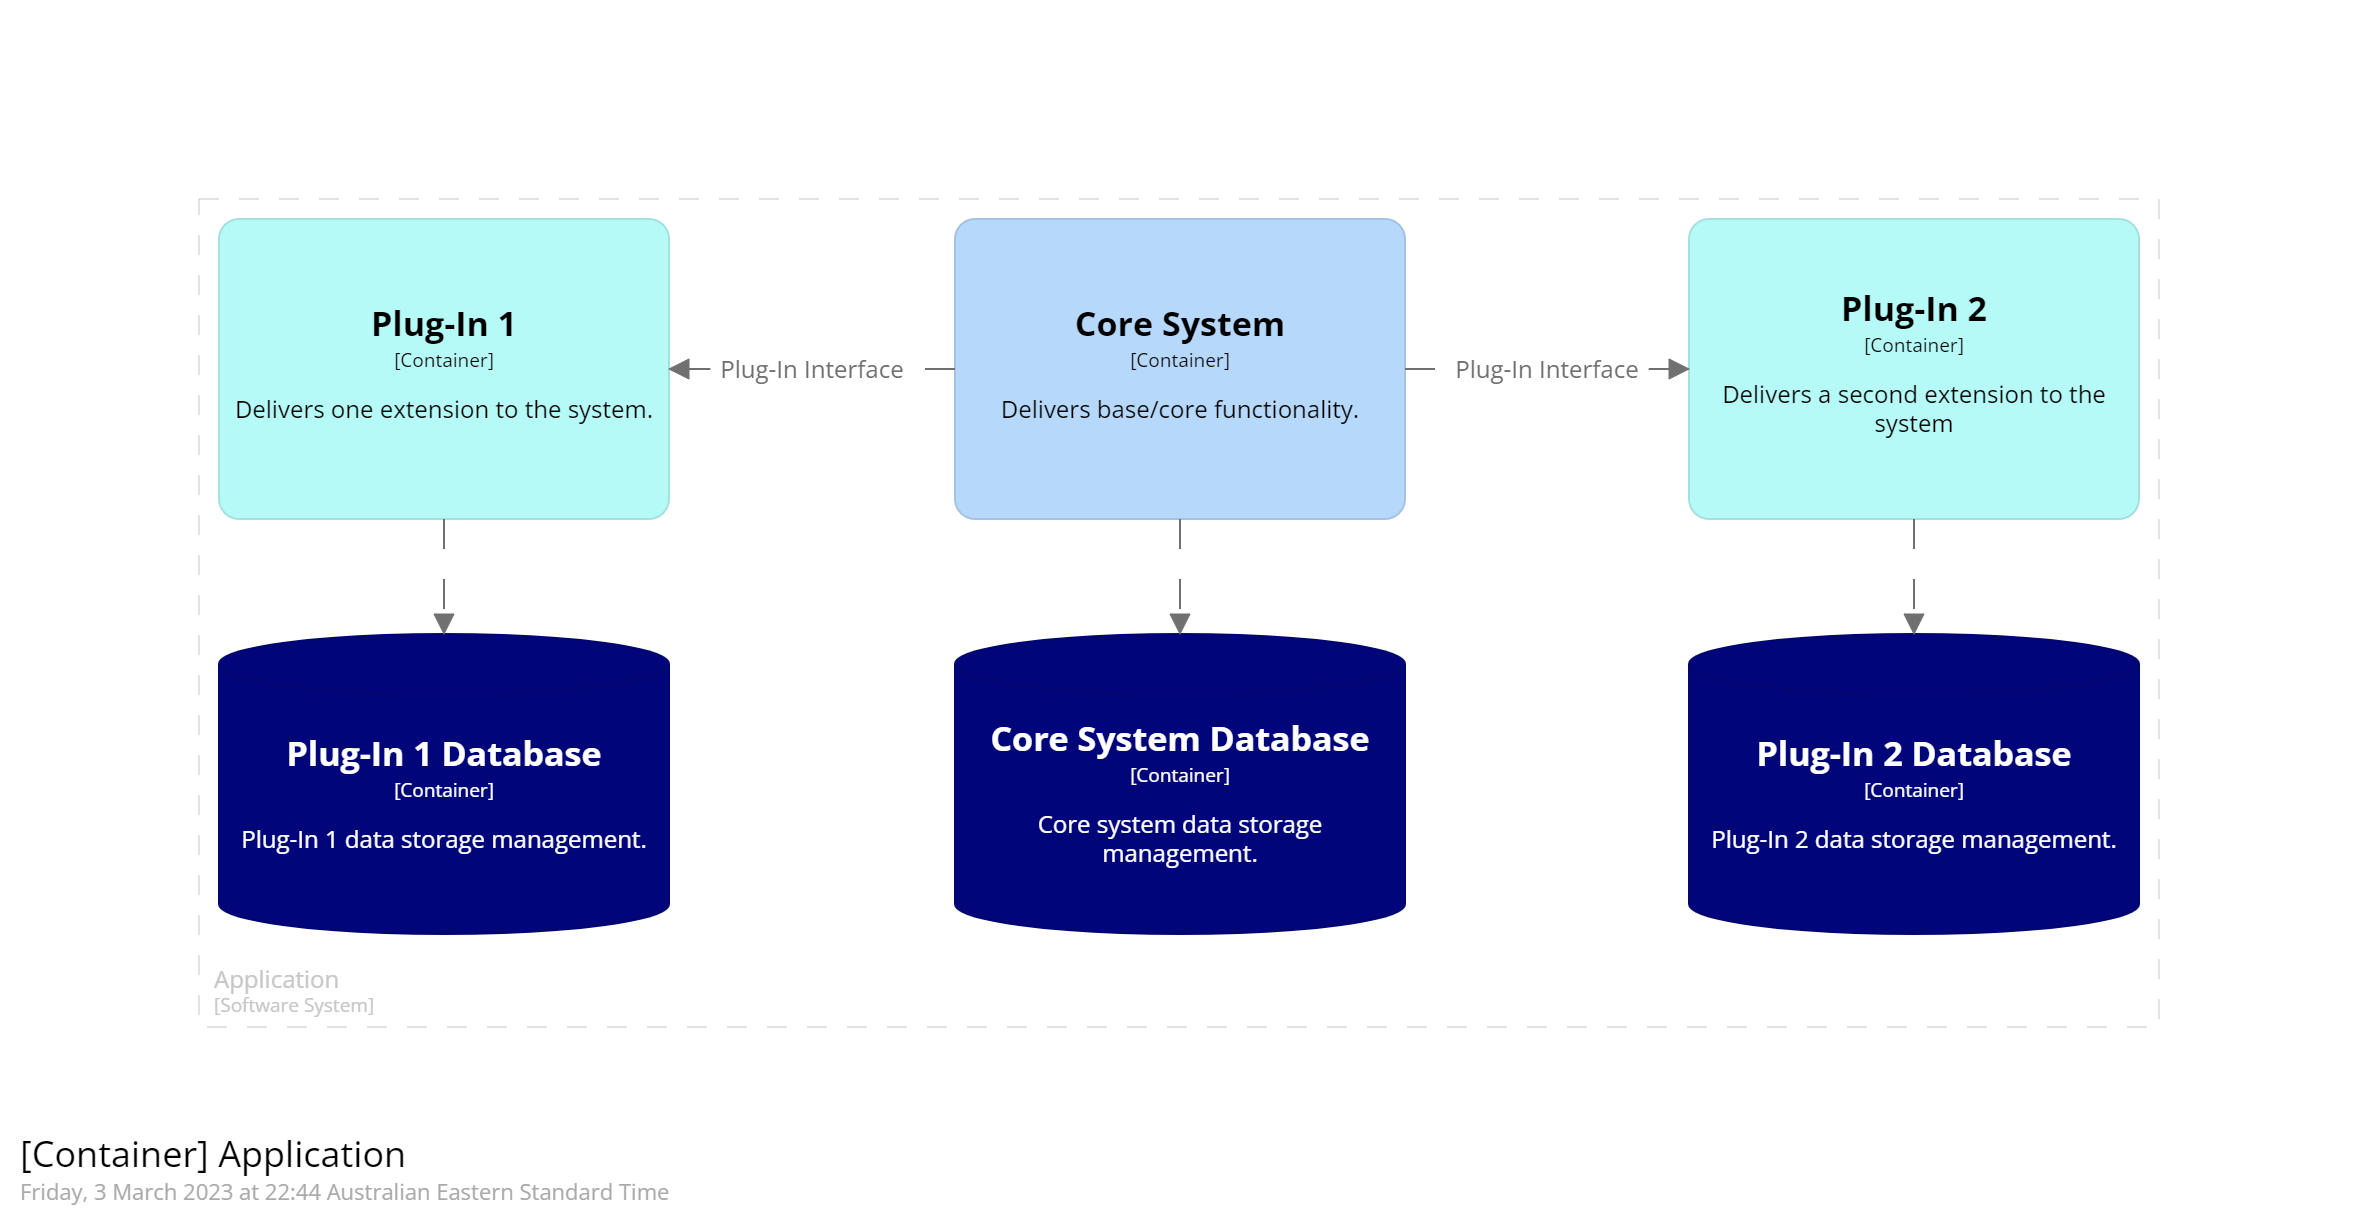
\includegraphics[trim=38 81 24 50,clip,width=\textwidth]{../../notes/microkernel/diagrams/plug-in-databases.png}
\end{frame}

\begin{frame}{Plug-ins as External Services}
    \begin{itemize}
        \LARGE\item Need communication protocol
        \LARGE\item Registry records communication contract
        \begin{itemize}
            \Large\item e.g. URL of the REST endpoint \& data passed to it
        \end{itemize}
    \end{itemize}
    \vspace{1cm}
    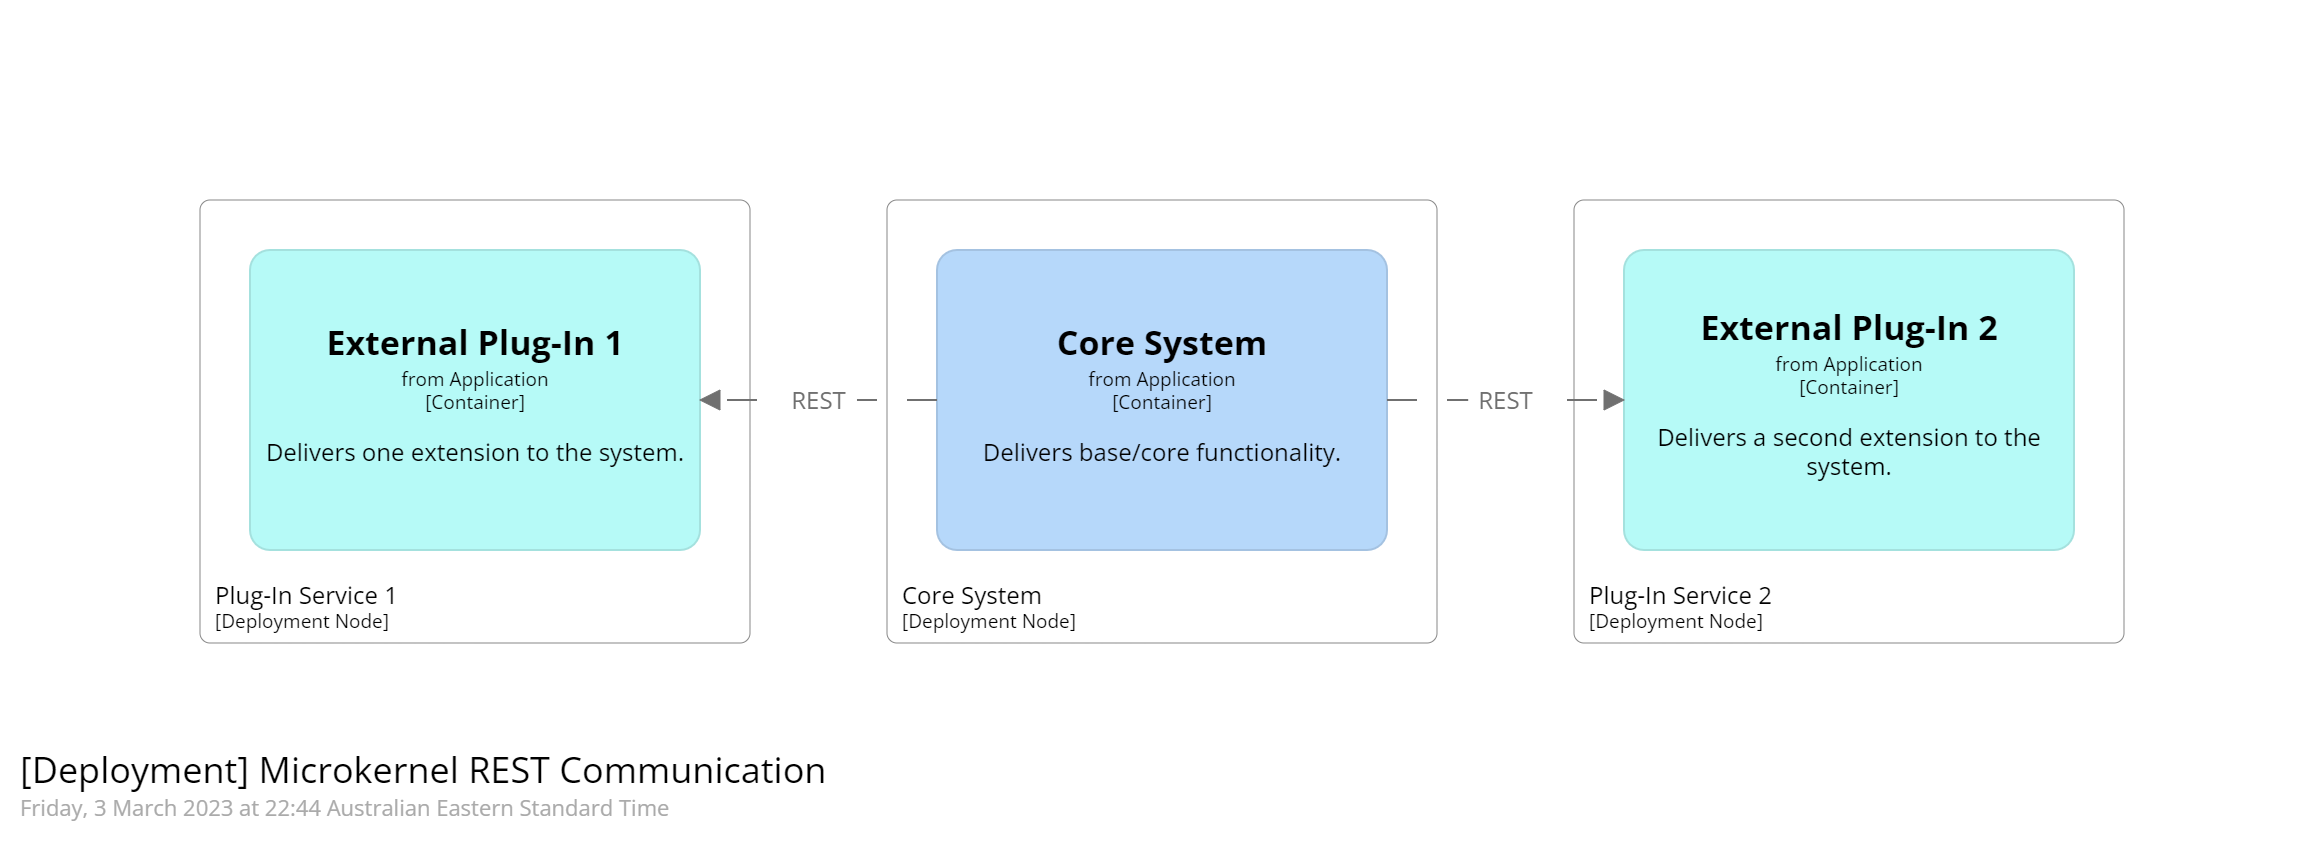
\includegraphics[trim=38 167 19 45,clip,width=\textwidth]{../../notes/microkernel/diagrams/rest-microkernel.png}
\end{frame}
\note[itemize]{
    \item May be deployed on same or separate infrastructure
    \item Allows broad range of communication protocols
}

\begin{frame}{Adapting Non-Conforming Interfaces}
    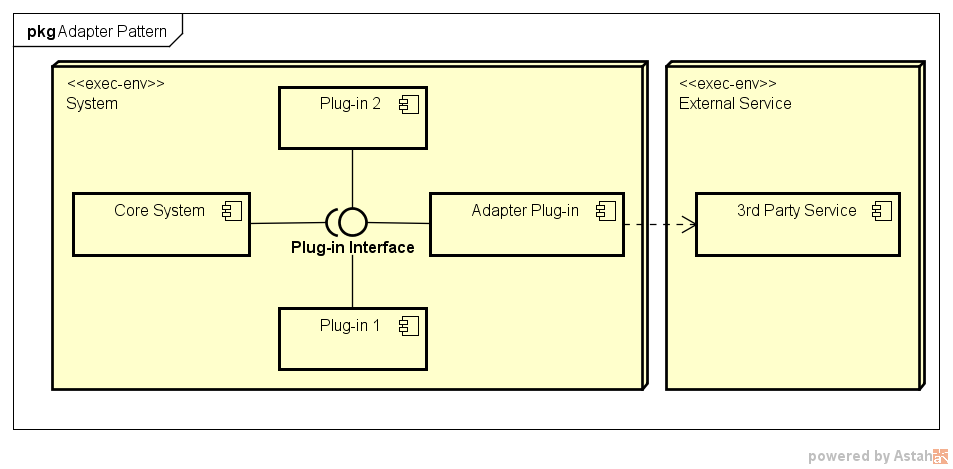
\includegraphics[trim=38 58 20 45,clip,width=\textwidth]{../../notes/microkernel/diagrams/adapter-plug-in.png}
\end{frame}
\note{Introduce \emph{adapter} design pattern as approach to manage 3rd party services as plug-ins}

\begin{frame}
    \vspace{4mm}
    \begin{columns}[t]
    \column<1->{0.5\textwidth}
        \centering
        \LARGE Technical Partitioning
        \begin{figure}
            \centering
            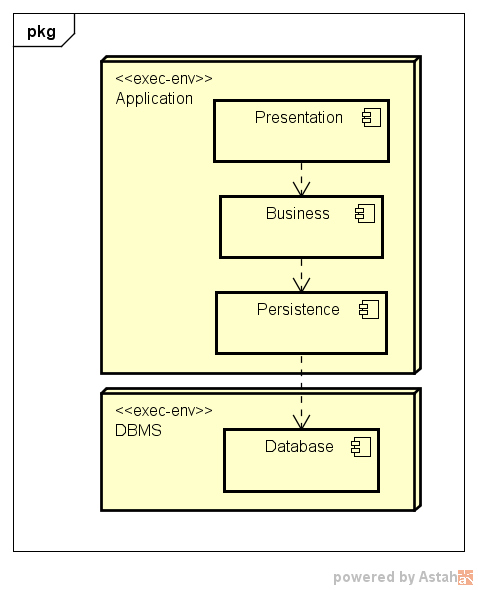
\includegraphics[trim=30 50 142 45,clip,width=0.35\textheight]{diagrams/technical-partitioning.png}
        \end{figure}
    \column<2->{0.5\textwidth}
        \centering
        \LARGE Domain Partitioning
        \begin{figure}
            \centering
            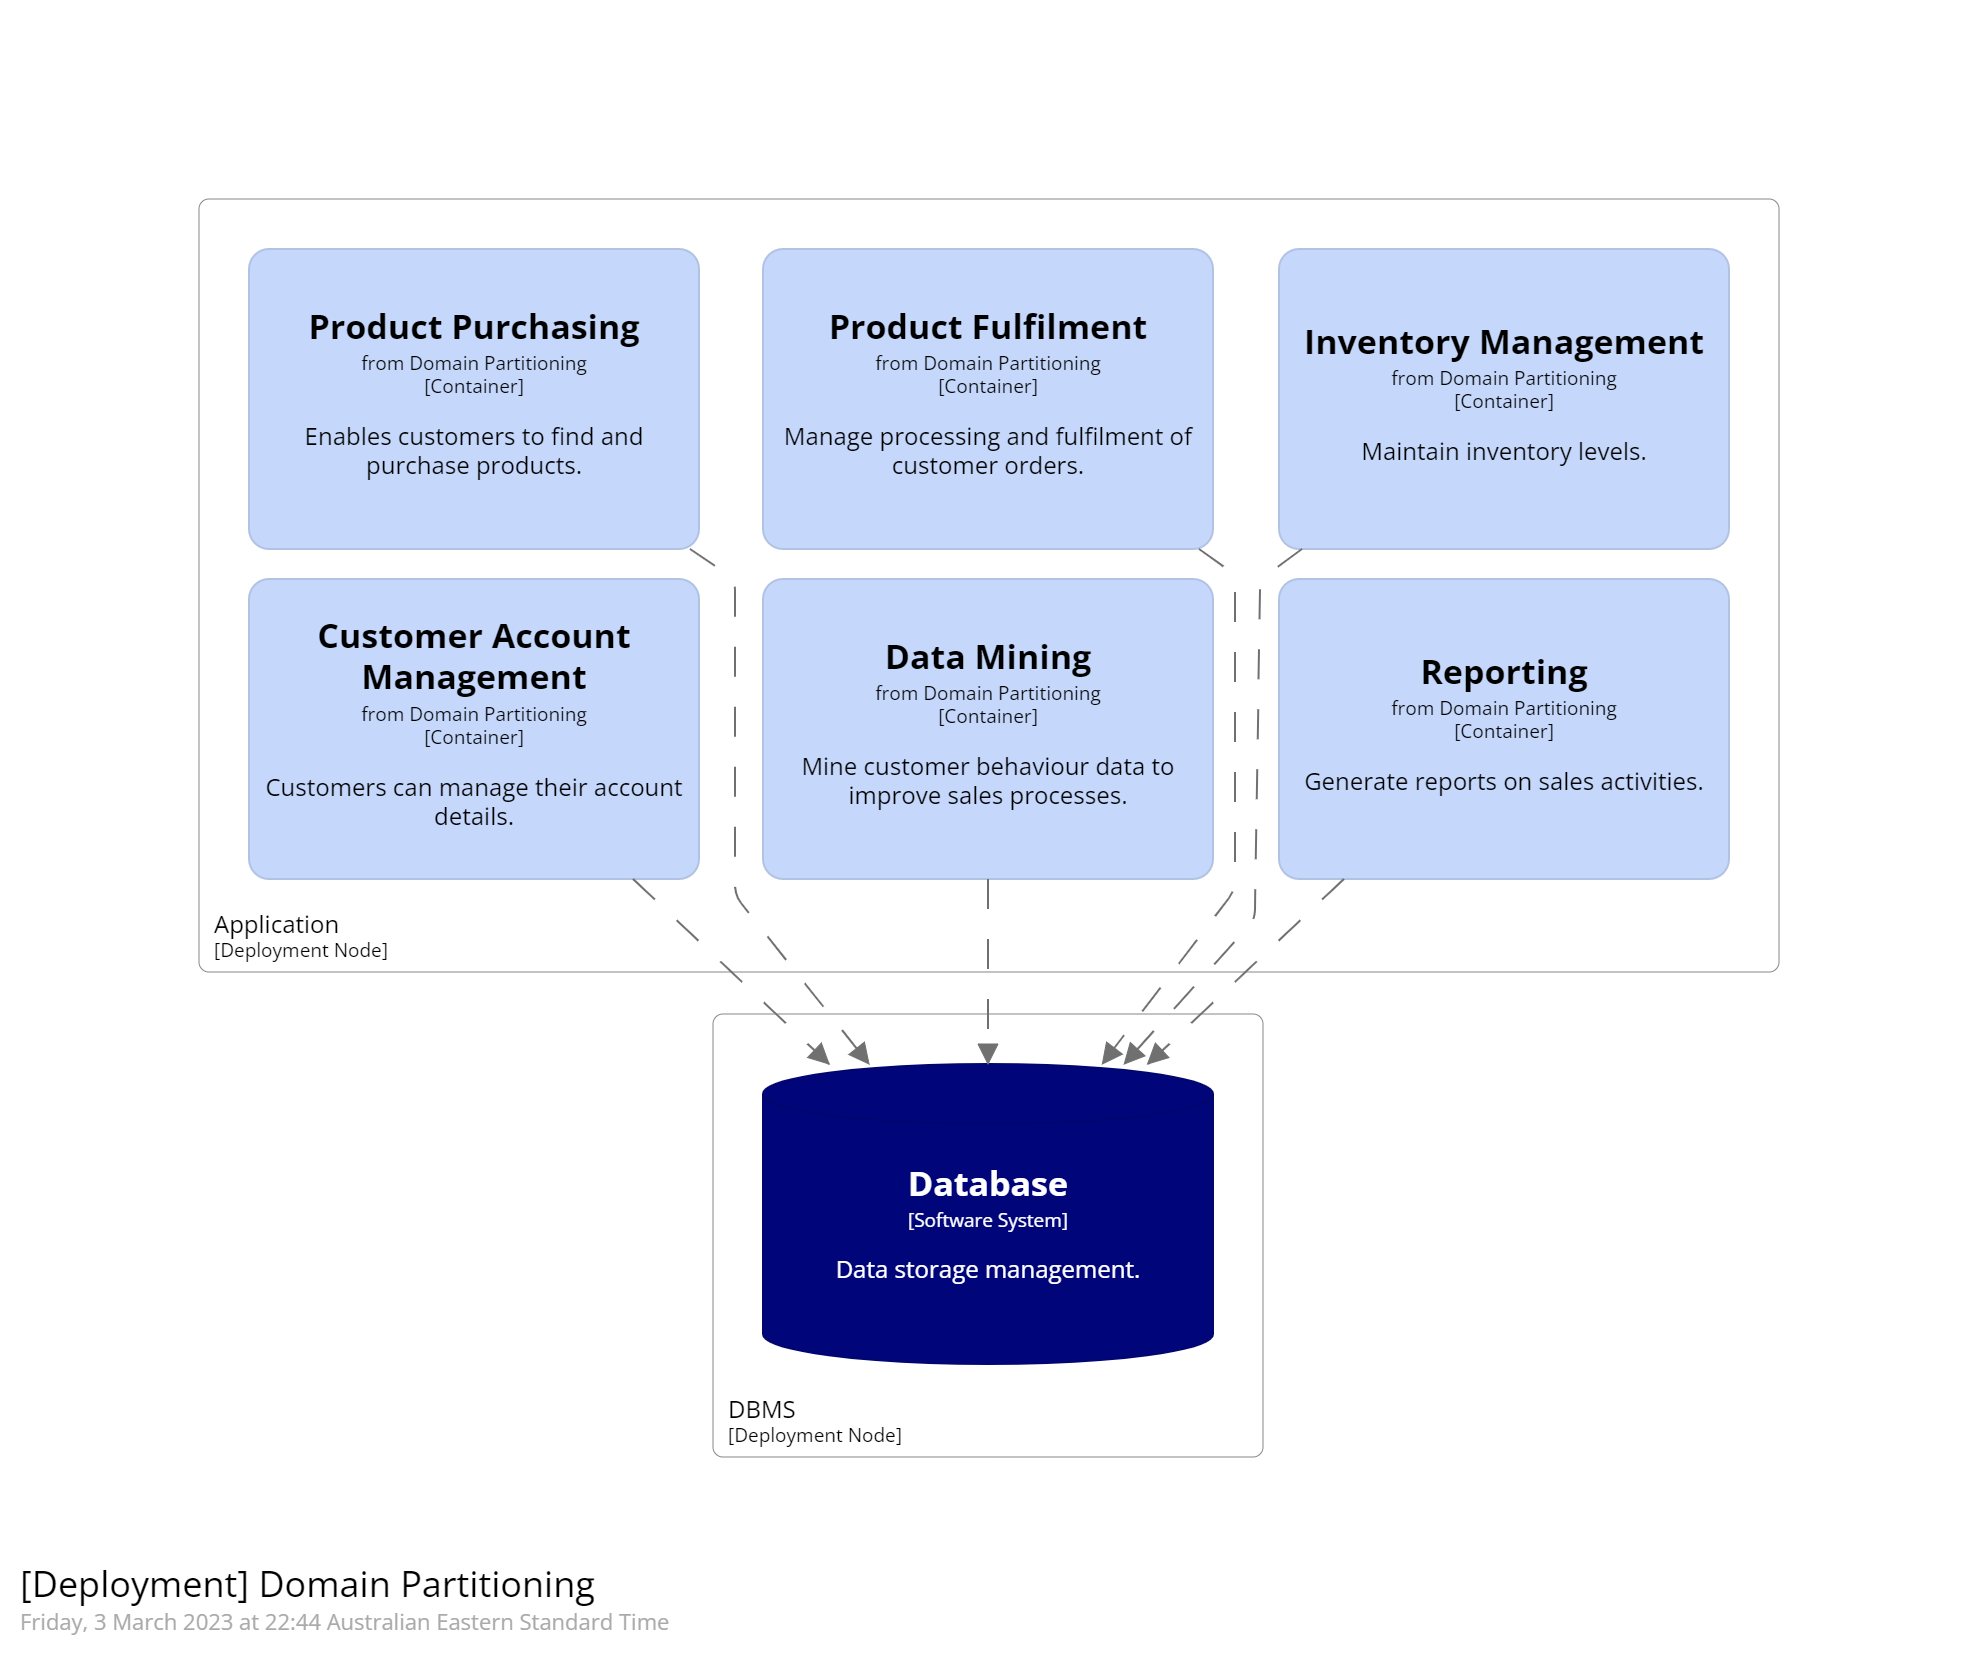
\includegraphics[trim=38 50 19 45,clip,width=\textwidth]{diagrams/domain-partitioning.png}
        \end{figure}
    \end{columns}
\end{frame}
\note[itemize]{
    \item Summarise differences between technical and domain partitioning
    \item Review layered architecture as technical partitioning
    \begin{itemize}
        \item Emphasise it is not the only way to perform technical partitioning
    \end{itemize}
    \item Example of on-line store partitioned into domains
}

\questionanswer{Is the microkernel architecture suited to \highlight{technical} or \highlight{domain} partitioning?}
{Core system can be partitioned either way.}

\begin{frame}{Domain Standard Interfaces}
    \vspace{3mm}
    \centering
    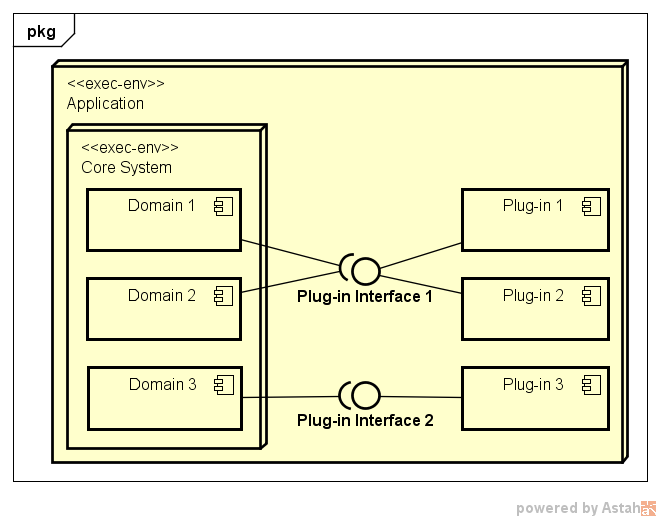
\includegraphics[trim=38 42 23 42,clip,width=1.25\textheight]{../../notes/microkernel/diagrams/domain-microkernel.png}
\end{frame}
\note[itemize]{
    \item Each domain can have its own plug-in interface
    \item Some domains may share a plug-in interface
}

\begin{frame}{Distributed Microkernel}
    \begin{itemize}
        \LARGE\item Partitions in the core system can be distributed
        \begin{itemize}
            \Large\item Technical or domain partitions
            \Large\item Plug-ins could also be distributed
        \end{itemize}
    \end{itemize}
    \vspace{3mm}
    \centering
    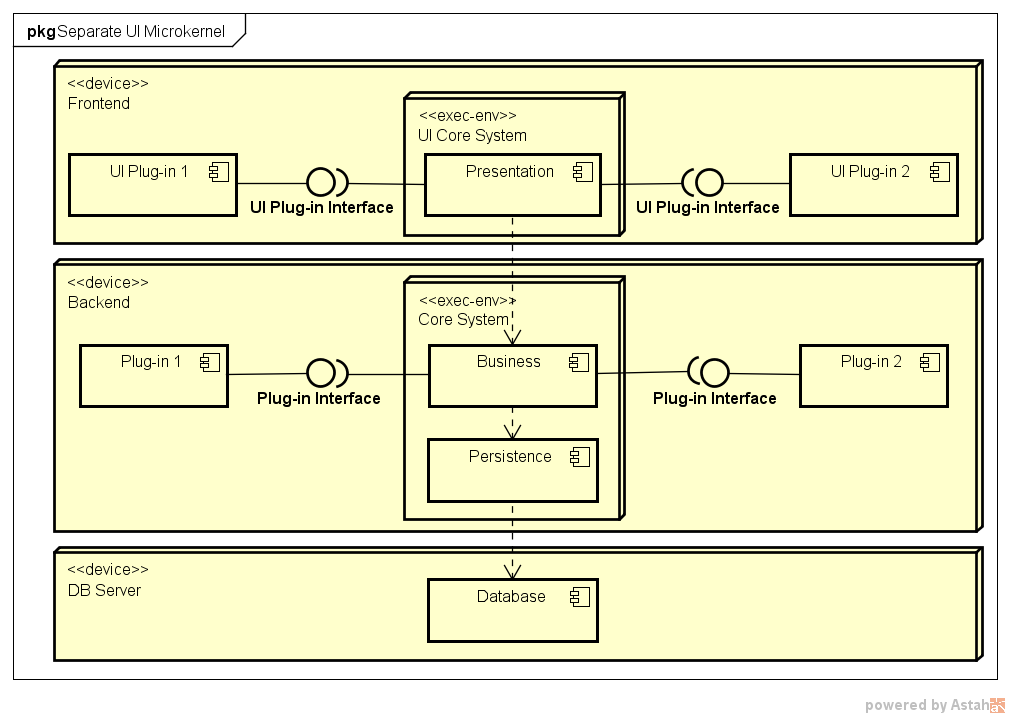
\includegraphics[trim=39 138 19 43,clip,width=0.7\textwidth]{../../notes/microkernel/diagrams/separate-ui-microkernel.png}
\end{frame}
\note{Comment on additional complexity}

\begin{frame}{Pros \& Cons}
    \vspace{1mm}
    {\huge
    \begin{description}
        \item[Simplicity] Core system \& Plug-in interface \tabto{15em}
\includegraphics[width=10mm]{../../shared/images/thumbs-up.png}
        \item[Extensibility] Plug-ins \tabto{15em}
\includegraphics[width=10mm]{../../shared/images/thumbs-up.png}
        \item[Interoperability] Plug-ins \tabto{15em}
\includegraphics[width=10mm]{../../shared/images/thumbs-up.png}
        \item[Scalability] \tabto{15em}
\includegraphics[trim=22 19 22 15,clip,width=10mm]{../../shared/images/thumbs-down.png}
        \item[Reliability] \tabto{15em}
\includegraphics[trim=22 19 22 15,clip,width=10mm]{../../shared/images/thumbs-down.png}
    \end{description}
    }
\end{frame}

\end{document}